\section{Interference/Coherence}
When we think of interference we think of things like the double slit, and michelson-morley experements.

In order to probe coherence we consider young's experement, where we filter to two points from a single light source. For something like the sun we have two sources that aren't physically connected.
In this experiment we will measure the intensity of light averaged over time. Expressed mathematically we measure:
\begin{align*}
	\int_{t-\frac{T}{2}}^{t+\frac{T}{2}} |E(t')|^2 dt'
\end{align*}
Where our detecter bandwidth is $\frac{1}{T}$. This could be changed to be related to some windowing function instead, where this detector is the detector generated by a tophat function.
If we have two different $E$ fields from our source we can say our irradiance is:
\begin{align*}
	I &= \int_{t-\frac{T}{2}}^{t+\frac{T}{2}} |E(t')|^2 dt' \\
	I &= \int_{t-\frac{T}{2}}^{t+\frac{T}{2}} |E_1(t') + E_2(t')|^2 dt' \\
	I &= I_1(t) + I_2(t) + 2\Re{\int dt E_1^* E_2} \\
	\int dt' E_1^* E_2 &= \int dt' |E_1| e^{-i\phi_1} |E_2| e^{i\phi_2} \\
	\int dt' E_1^* E_2 &= \int dt' |E_1| |E_2| e^{i\Delta \phi_{12}}
\end{align*}
Which if $\phi_1$ and $\phi_2$ are uncorrelated, then we should have no interference term. We think of light from the sun as random so we expect there to be no interference term, or in other words no coherence.

In this context when we talk about coherence we mean fixed phase relationships between two different fields.

\begin{figure*}[h]
	\centering
	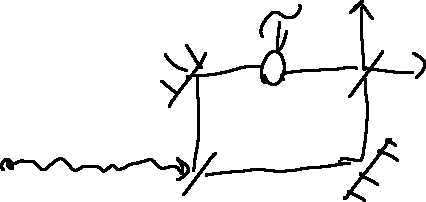
\includegraphics[width=6cm]{2-10-1.png}
	\caption*{Mach-Zender}
\end{figure*}
Now we consider splitting our point source at a beam splitter and then recombining it in a ``Mach-Zender'' interferometer, which we see will give us:
\begin{align*}
	E_\text{up} &= -rr'E_1(t+\tau) + tt' E_1(t) \\
	E_\text{r} &= tr' E_1(t) + rt' E_1(t+\tau)
\end{align*}
If we now choose 50/50 beam splitters so $r=t=\frac{1}{\sqrt{2}}$:
\begin{align*}
	E_\text{up} &= \frac{1}{2}(E_1(t) - E_1(t+\tau)) \\
	E_\text{r} &= \frac{1}{2} (E_1(t) + E_1(t+\tau))
\end{align*}
S o our irradiance in this situation becomes:
\begin{align*}
	I_r(t,\tau) &= \frac{1}{4} \int dt' \left[|E_1(t')|^2 + |E_1(t' + \tau)|^2 + 2\Re{|E_1(t')||E_1(t' + \tau)| e^{i(\phi_1(t') - \phi_1(t'+\tau))}}\right]
\end{align*}
In order to analyze this we now look at this in the fourier domain (we vary $\tau$ and then do a fourier transform in an experiment) here we will remove the terms that don't correspond to the coherences, 
potentially by simply measuring them and canceling them, or by ignoring the low frequency components:
\begin{align*}
	\tilde{I}_r(t,\omega) &= \int e^{i\omega\tau} I_r(t,\tau) d\tau \\
	\tilde{I}_r(t,\omega) &= \frac{1}{4}\int d\tau e^{i\omega\tau} \int dt'(2|E_1(t')||E_1(t'+ \tau)|\cos \Delta\phi_{12}(t';\tau) + \omega_0\tau
\end{align*}
Where $\omega_0$ is the wave's ``carrier'' frequency.
\begin{align*}
	\tilde{E}(\omega) &= A(\omega-\omega_0) & A(\omega) &= \mathcal{F}(|E_(t)|) \\
	\tilde{I}_r(t,\omega) &= \frac{1}{2}\int d\tau e^{i\omega\tau} \int dt'\Re(E_1^*(t')E_1(t'+ \tau)) \\
	\tilde{I}_r(t,\omega) &= \frac{1}{2}\int d\tau e^{i\omega\tau} \int dt'\Re\left(\int \frac{d\omega'}{2\pi} e^{i\omega't'} \tilde{E}(\omega')\int \frac{d\bar{\omega}}{2\pi} e^{-i\bar{\omega}(t'+\tau)} \tilde{E}^*(\bar{\omega})\right) \\
	\tilde{I}_r(t,\omega) &= \frac{1}{2}\Re\left(\int \frac{d\omega'}{2\pi}\int \frac{d\bar{\omega}}{2\pi} \int dt'e^{i(\omega' - \bar{\omega})} \tilde{E}(\omega')  \tilde{E}^*(\bar{\omega})\int d\tau  e^{i\tau(\omega-\bar{\omega})}\right) \\
	\tilde{I}_r(t,\omega) &= \frac{1}{2}\Re\left(\int d\omega'\int d\bar{\omega} \delta(\omega' - \bar{\omega}) \tilde{E}(\omega')  \tilde{E}^*(\bar{\omega})\delta(\omega-\bar{\omega})\right) \\
	\tilde{I}_r(t,\omega) &= \frac{1}{2}\Re\left(\tilde{E}(\omega)  \tilde{E}(\omega)\right) \\
	\tilde{I}_r(t,\omega) &= \frac{1}{2}|\tilde{E}(\omega)|^2
\end{align*}
Which gives us a spectral intensity of our light. This relation is the ``Weiner-Khinchin'' theorem. We call $\expval{E^*(t)E(t+\tau)}$ the first order correlation function. The Weiner-Khinchin theorem explicitly says:
\begin{align*}
	\expval{|\tilde{E}(\omega(|^2} &= \mathcal{F}(\expval{E^*(t)E(t+\tau)})
\end{align*}
We add quantum to this picture by replacing our field amplitudes here into operators
\subsection{Degree of first order coherence}
\begin{align*}
	g_{ij}^{(1)} (\tau,r) &= \frac{\expval{\hat{E}_i^{(-)}(x,t)\hat{E}_j^{(+)}(x+ r,t+\tau)}}{\sqrt{I_i(x,t) I_j(x+r,t+\tau)}}
\end{align*}
Describes our coherences, where $i,j$ label our polarizations/modes and this is an implicit function of $x,t$. Looking at fixed positions we can see this becomes:
\begin{align*}
	g^{(1)}(t,\tau) &= \frac{\expval{\hat{E}_i^{(-)}(t)\hat{E}_j^{(+)}(t+\tau)}}{\sqrt{I_i(t) I_j(t+\tau)}}
\end{align*}
If we have a stationary distribution, or if we have a detector that averages over the entire pulse length, then we have:
\begin{align*}
	g^{(1)}(\tau) &= \frac{\expval{\hat{E}_i^{(-)}(0)\hat{E}_j^{(+)}(\tau)}}{\sqrt{I_i(0) I_j(\tau)}}
\end{align*}
Which we write as:
\begin{align*}
	g^{(1)}(\tau) &= \frac{\expval{\hat{a}^\dagger(t)\hat{a}(t+\tau)}}{\sqrt{\expval{\hat{a}^\dagger(t)\hat{a}}\expval{\hat{a}^\dagger(t+\tau)\hat{a}(t+\tau)}}}
\end{align*}
Which will tell us about the spectrum of our source. On the other hand $g^{(1)}(x,t,r,\tau)$ tells about the modes of the source. This will not tell about the state of the field. To illustrate this we consider a single photon and a coherent state occupying the same mode:
\begin{align*}
	\hat{a}(t)\ket{1}_\psi &= \int dt' \hat{a}\hat{a}^\dagger \phi(t') \vac \\
	\hat{a}(t)\ket{1}_\psi &= \int dt' \delta(t-t') \phi(t') \vac \\
	\hat{a}(t)\ket{1}_\psi &= \phi(t) \vac
\end{align*}
So we can say:
\begin{align*}
	\expval{\hat{a}^\dagger(t) \hat{a}(t+\tau)} &= \psi^*(t)\psi(t+\tau) \\
	g^{(1)}(\tau) &= \frac{\psi^*(t)\psi(t+\tau)}{\sqrt{|\psi(t)|^2|\psi(t+\tau)|^2}}
\end{align*}
We repeat this for the coherent state:
\begin{align*}
	\expval{\hat{a}^\dagger(t)\hat{a}(t+\tau)} &= \psi^*(t)\psi(t+\tau)|\alpha|^2 \\
	g^{(1)}(\tau) &= \frac{\psi^*(t)\psi(t+\tau)|\alpha|^2}{|\alpha|^2\sqrt{|\psi(t)|^2|\psi(t+\tau)|^2}}\\
	g^{(1)}(\tau) &= \frac{\psi^*(t)\psi(t+\tau)}{\sqrt{|\psi(t)|^2|\psi(t+\tau)|^2}}
\end{align*}
\subsection{Degree of 2nd order coherence}
So far we have only extracted information about the modes that we are occupying. The first order coherence can be thought of as containing information about amplitude correlations.
We will now look at the intensity correlations, which will tell us about the states in the modes.
These are related to Hanbury-Brown and Twiss experiment, which let us measure the diameters of stars without using interferometers.

We define:
\begin{align*}
	g^{(2)}(\tau) &= \frac{\expval{\hat{a}^\dagger(t)\hat{a}^\dagger(t+\tau)\hat{a}(t+\tau)\hat{a}(t)}}{\expval{\hat{a}^\dagger(t)\hat{a}}\expval{\hat{a}^\dagger(t+\tau)\hat{a}(t+\tau)}}
\end{align*}
We measure this using something like a Hanbury-Brown Twiss setup.
\begin{figure*}[h]
	\centering
	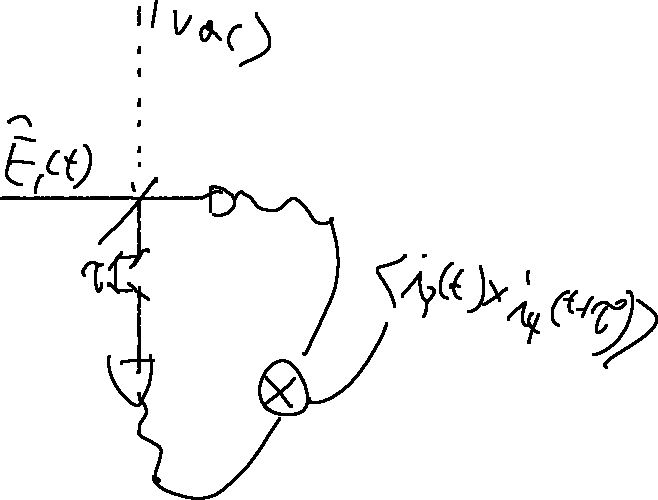
\includegraphics[width=6cm]{2-10-2.png}
	\caption*{Hanbury-Brown Twiss}
\end{figure*}

Our measurement will be:
\begin{align*}
	\expval{\hat{I}_3(t) \hat{I}_4(t+\tau)}
\end{align*}
If we input a single photon state we find after the beam splitter our state is:
\begin{align*}
	\ket{\psi} &= \frac{1}{\sqrt{2}}(\ket{1}_3\ket{0}_4 + \ket{0}_3\ket{1}_4)
\end{align*}
So then:
\begin{align*}
	\expval{\hat{a}_3^\dagger(t)\hat{a}^\dagger_4(t+\tau)\hat{a}_4(t+\tau)\hat{a}(t)} &= 0
\end{align*}
In contrast a coherent state gives us:
\begin{align*}
	\expval{\hat{a}_3^\dagger(t)\hat{a}^\dagger_4(t+\tau)\hat{a}_4(t+\tau)\hat{a}(t)} &= \frac{1}{4} \expval{(\hat{a}_1^\dagger(t) - \hat{a}_2^\dagger(t))(\hat{a}^\dagger_1(t+\tau) +\hat{a}^\dagger_2(t+\tau) +\ldots}
\end{align*}
If we drop all $\hat{a}_2$ terms since we have assumed that our starting state for the 2 modes is $\vac$, so we have:
\begin{align*}
	\expval{\hat{a}_3^\dagger(t)\hat{a}^\dagger_4(t+\tau)\hat{a}_4(t+\tau)\hat{a}(t)} &= \frac{1}{4} \expval{\hat{a}_1^\dagger(t)\hat{a}^\dagger_1(t+\tau)\hat{a}_1(t+\tau)\hat{a}_1(t)}
\end{align*}
If we input a coherent state we find:
\begin{align*}
	\expval{\hat{a}_3^\dagger(t)\hat{a}^\dagger_4(t+\tau)\hat{a}_4(t+\tau)\hat{a}(t)} &= \frac{1}{4} |\alpha|^4 |\psi(t)|^2|\psi(t+\tau)|^2
\end{align*}
And dividing by the normalizations we see:
\begin{align*}
	g^{(2)}(\tau) &= \frac{|\alpha|^4 |\psi(t)|^2|\psi(t+\tau)|^2}{|\alpha|^4 |\psi(t)|^2|\psi(t+\tau)|^2} \\
	g^{(2)}(\tau) &= 1
\end{align*}
We note:
\begin{align*}
	g^{(2)} &= 0 & \text{single} \\
	g^{(2)} &= 1 & \text{coherent} \\
	g^{(2)} &= 2 & \text{thermal} \\
	g^{(2)} &\geq 2 & \text{squeezed}
\end{align*}
